\chapter{Energetic Electron Precipitation and Geospace}

\section{Introduction to Connected Geospace}

The Earth is a complicated place. Natural processes, which occur on vastly different time scales, are all connected to each other and produce the state of the overall system. Only in the last 70 years or so, since the beginning of the space age, has the picture of the Earth as a dynamic system been extended to include the space around it. This space is not empty, and it has structure and dynamics which are very different than processes on Earth, mostly owing to the importance of the electromagnetic force between its constituents. The word used to describe the space around Earth is geospace, so-named because the Earth and its processses are not strictly separated from the space around it. In fact, information, matter, and energy flow between regions which can be separated by great distances, and cause effects which can echo throughout the entire system. In this chapter, I will describe one of the most dramatic ways which this can happen, where energetic particles from space enter the atmosphere and affect it directly. 

Energetic electron precipitation is a process by which electrons depart trapped states in geospace and enter the Earths atmosphere. One of the most brilliant effects that can be caused by this process is able to be seen from the ground on Earth - the northern lights, or Aurora Borealis. There has been a great deal of work done in the last half-century to understand, quantity, and model the processes responsible for creating the Aurroa, but many unanswered questions remain. With the knowledge that the Earth and the space around it are both connected and affect each other, it becomes of great scientific interest to understand the ways which particles and energy move between them. The fact that energetic particle precipitation can have dramatic visual affects on the atmosphere motivates its use as measurable target which can provide a window to the dynamics of the connected system. 

The earth and geospace are not stationary systems. One can draw a loose analogy between their related structure and the anatomy of a living organism. While the system is always in a state of change, there is a consistent structure and organization at the highest levels. In this case, that structure is largely defined by the magnetic field of the Earth, and the magnetic field of the solar wind which interacts with it. Navigation on the surface of the Earth can be accomplished by measuring the direction of the local magnetic field in two dimensions. In geospace, the magnetic field changes significantly over all three dimensions, and, to an extent, in time as well. As charged particles, electrons in geospace are subject to the Lorentz force. This force is always orthogonal to the magnetic field, which is why the magnetic field is such a powerful organizational force in the system. 

The magnetic field of the Earth is due to both internal, and external (space-based) current sources. This field can be conveniently described by the multipole expansion. Figure~\ref{magnetosphere_diagram} shows a model of the magnetic field of the Earth, which takes into account both internal and external sources. Towards the surface, the dipole is a good approximation. Farther away, however, higher-order terms become important and result in a field has a vastly different structure than the dipole description. The magnetic field geometry in Figure~\ref{magnetosphere_diagram} does not imply a steady-state to the system. Rather, this can be thought of as the overall topology of a system which is always in motion. In reality, only some modified version of this picture will be accurate at any particular time. Particularly, at distances which exceed a few Earth radii, the state of the solar wind, through which the Earth is always moving, becomes more important than the current sources internal to the Earth itself. A more accurate picture of the system than Figure~\ref{magnetosphere_diagram} would actually be an animation, with magnetic field lines cascading on the dipole field of the Earth, and reconnecting to form the stretched-out ``tail'' from 10 to hundreds of Earth radii ``downwind''. The description of that process is an entire field of study, and it too, has questions which are currently unanswered.

\begin{figure}[p]
\label{magnetosphere_diagram}
\centering
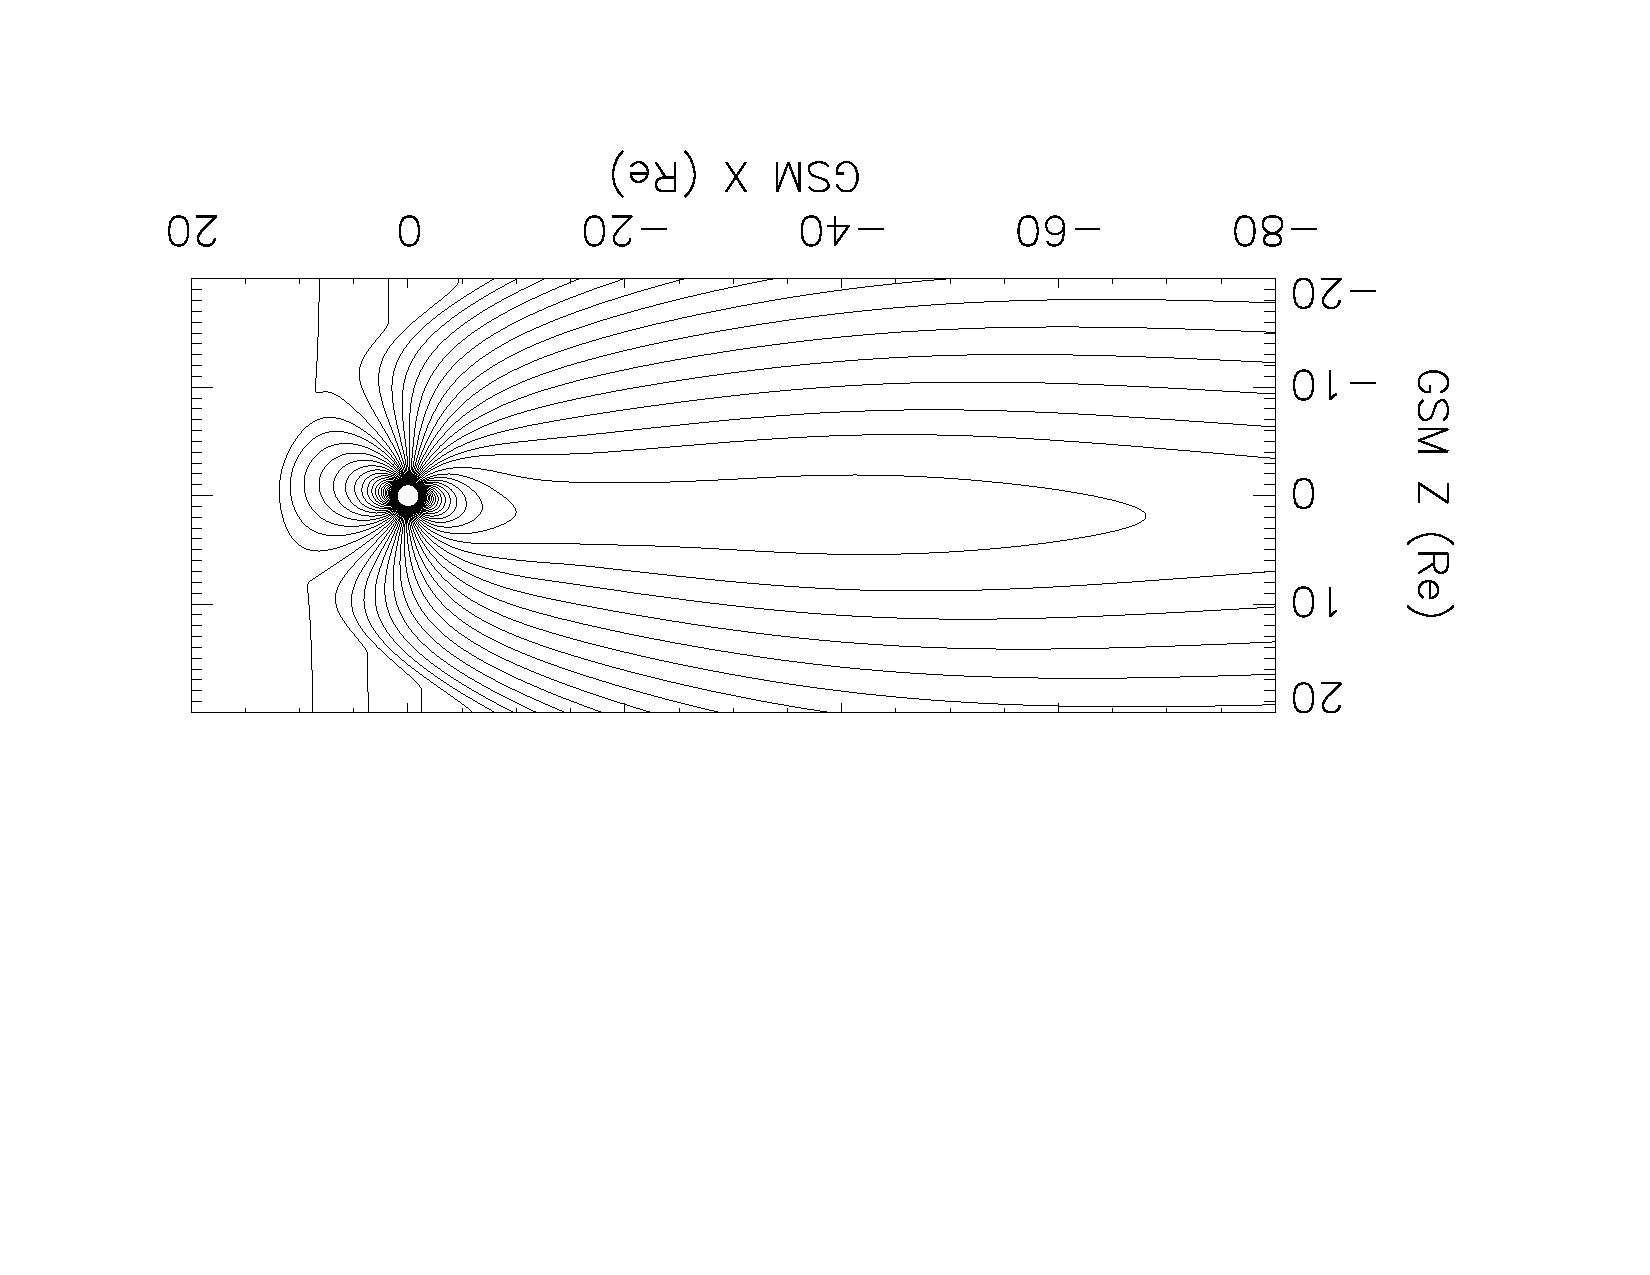
\includegraphics[width=1.1\textwidth,angle=180]{figures/chapter_2/magnetosphere_diagram/magnetosphere_diagram}
\caption{Model of the magnetic field of the Earth which includes effects due to external sources and the solar wind. Coordinates are measured in Earth radii and centered on the Earth. Near to the earth, a dipole field describes the geometry well. Farther away, this changes. }
\end{figure}

Given that electrons in geospace exist, and they are subject to a magnetic field geometry which is complicated and dynamic on the relevant scales, this suggests that the motion of electrons within the system is important to the state of the overall system. This, then, implies that the loss of these particles to the Earths atmosphere, is also important. The goal of this chapter is to describe, in adequate detail, the connection between the precipitation of electrons into the atmosphere and the state of the larger geophysical system. The goal is to advance electron precipitation, which is a fairly dramatic event, as a process which is both worth understanding in its own right, but also as a tool, which provides a window in to the processes which occur in the larger system. 

\section{Electrons in Geospace}

The first American artificial satellite, Explorer 1, was launched in 1958. Among other instruments, it carried a Geiger counter, which is a device sensitive to the energy deposition of charged particles like electrons. The expected background count rate due to cosmic rays was observed at some points during the flight, but at others, zero counts were reported. This was determined on later flights, to be due to the saturation of the device by a much larger than expected radiation flux. This led to the discovery of the radiation belts around the Earth. The question then became why the radiation belts existed, and what their properties are. A review of the historical development of knowledge about the radiation belts is~\cite{baker2012}. 

The radiation belts have a spatial structure. This is shown in Figure~\ref{radbelts_structure}, which is an evaluation of a model, AE9, generated from measurements from many different satellites (see~\cite{ginet2013}). An approximate description of the Earths magnetic field~\citep{tsyganenko97} is overlaid to show that the it is the main geometry at play. There are three essential regions. The inner zone, and outer zone are distinct and separated by a region of empty space, called the slot region.

\begin{figure}[p]
\label{radbelts_structure}
\centering
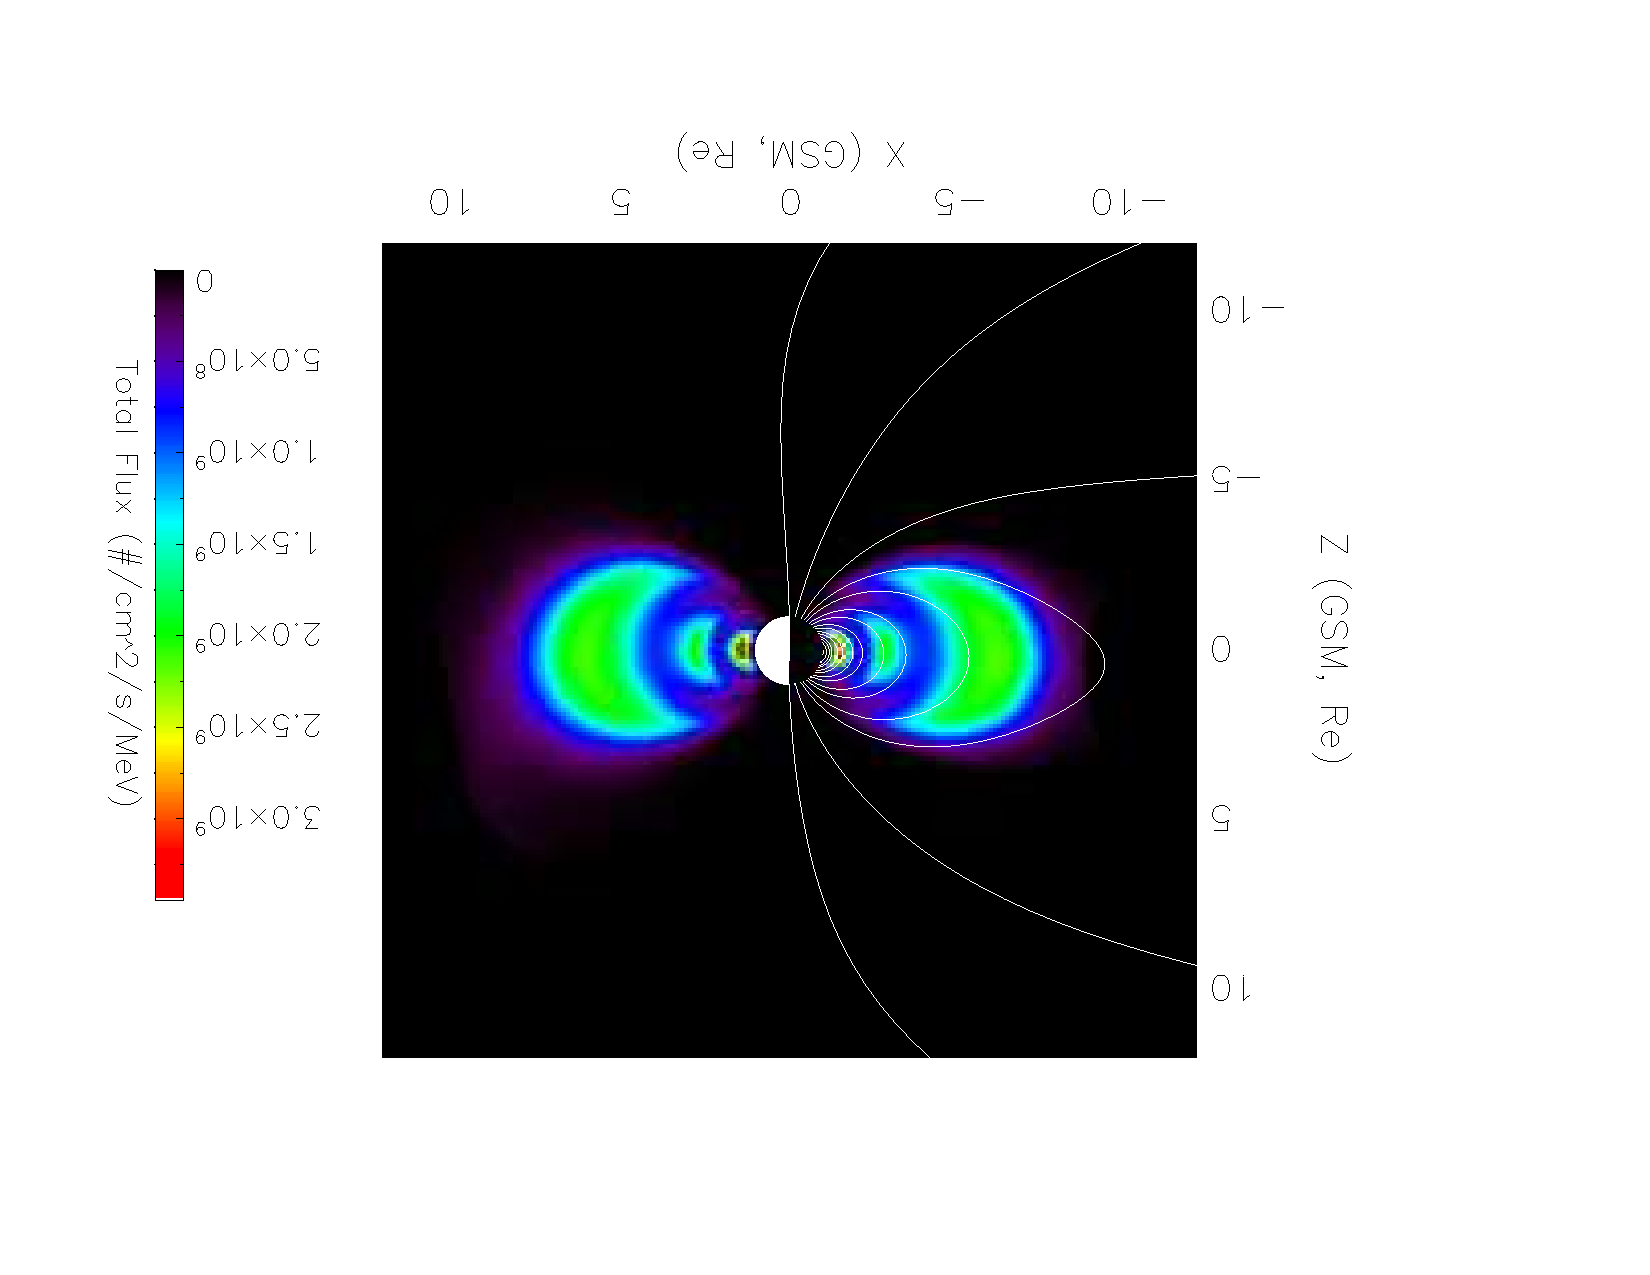
\includegraphics[width=1.0\textwidth,angle=180]{figures/chapter_2/radbelts_structure/radmodel}
\caption{Cutaway view of AE9 model electron fluxes in the radiation belts, with some model magnetic field lines from ~\cite{tsyganenko97} to show the overall geometry.}
\end{figure}

The main process which is thought to be responsible, at least partially, for the existsnce of the inner radiation belt is called cosmic ray albedo neutron decay (CRAND)~\citep{singer1958}. In the CRAND process, cosmic rays from space create neutrons in the upper atmosphere, which are then free to travel upwards, or downwards. Those which travel upwards, and subsequently decay into a proton and an electron, form the inner radiation belt. The gap that defines the separation of the inner and outer radiation belts is called the slot region, and is caused by a kind of radio wave called plasmaspheric hiss. As the radio wave interacts with particles trapped in the slot region it changes their motion in such a way that they precipitate and are lost in the Earth’s atmosphere. This process can be partially understood through the adiabatic description of trapped particle motion, which is discussed in the next section. Even though steady-state and adiabatic expressions of the process by which the slot region is formed make predictions that agree with experimental data, they do not form a complete description. 

 \section{Single Particle Motion}
 
 Some properties of the radiation belts, and electron precipitation, can be understood through a simplified picture of their dynamics which considers particles independently. In this description, particle motions do not affect each other, that is, we ignore the fact that a charged particle moving an an electromagnetic field also creates an electromagnetic field due to its own motion. This picture neglects the collective effects characteristic of space plasmas. As a simplified picture, though, it provides a useful framework in which to describe the mechanism and effects of particle loss to the atmosphere.

For the purposes of this description, electrons from the radiation belts are free to move under the influence of the Earths magnetic field. The Lorentz force, $\mathbf{F} = q(\mathbf{E} + \mathbf{v}\times\mathbf{B})$, where $q$ is the electron charge, $\mathbf{v}$ is the velocity vector, and $\mathbf{B}$ is the static magnetic field, is the only force which they are subjected to. This causes cycloidal motion about magnetic field lines. There is no component of the force parallel to the magnetic field, so the electron is trapped, to orbit the field line and drift along it at whatever parallel velocity it started with as long as $\mathbf{B}$ is constant. 

If we consider a phase-space, where the canonical momentum of the particle $P$ is along one axis, and the spatial coordinate $q$ is along another, then, under slow changes to the path integral:

$$\oint P dq$$

compared to the periodicity of the system, there will be an approximately constant quantity. This quantity is called an adiabatic invariant. For electron gyro motion around a magnetic field line, the associated invariant is:

$$J_1 = \frac{\mu v_{\perp}^2}{2B}$$

where m is the electron mass, $v_{\perp}$ is the electron speed perpendicular to the magnetic field, and B is the local magnetic field strength. Since the electron gyro frequency is fast (order of MHz in the ionosphere, KHz in the magnetosphere), this is a well conserved quantity, until one considers scattering by wave phenomena. In the situation where scattering is not occurring, electrons will increase their gyro frequency and perpendicular velocity as they enter regions of space with increasing magnetic field strength, such as occurs towards the magnetic poles of the Earth. The fact that the magnetic force does not do work has an important implication. When the gyro frequency of the particle increases, the component of the velocity which is parallel to the magnetic field decreases, to conserve the overall kinetic energy. Eventually, the electron can reach a point where all of the kinetic energy is due to the perpendicular component of the velocity. This will prevent the electron from going further into the intensifying magnetic field strength, and it will turn around, and mirror, heading in the opposite direction. Define the pitch angle, $\alpha$ as the angle between the electron velocity vector and the local magnetic field. If $B_0$ is the magnetic field strength at the equator, and $b_m$ is the local magnetic field strength, then the pitch angle is (from conservation of $\mu$):

$$\sin^2\alpha = B_0/B_m.$$

The electrons undergo gyro motion about magnetic field lines, and due to the invarant $J_1$, they bounce between the magnetic poles. This is called magnetic mirroring. The mirror height is the altitude above the surface of the Earth where the particles reverse direction. Any particle with a mirror height below the top of the atmosphere will be lost. The set of pitch angles for which electrons fail to mirror and enter the atmosphere is called the loss cone. 

The bounce-motion of electrons between hemispheres is itself periodic motion, and gives rise to another approximately conserved quantity. Choose the momentum coordinate to the along the magnetic field line with distance element $ds$, and the momentum to be the parallel component $mv_{\parallel}$. The associated invariant is then:

$$J_2 = \oint v_{\parallel}ds$$

for mirror-trapped electrons. The bounce time between mirror points for electrons in geospace is on the order of a few seconds, so this is a well-conserved quantity for processes that occur on any time scales longer than that. 

\section{Scattering Processes}

Single particle motion describes a picture of the radiation belts which accounts for their overall anatomy and steady-state behaviour. This picture changes when dynamic effects occur that cause particles to leave the system and precipitate to the atmosphere. In this section, we will give a high level description of how and why these processes occur, and what some of their known effects are. The emphasis will be on how these processes connect to the larger picture of geospace, rather than the details of the physics governing each one. We advance the idea that, as both a cause and a result of processes in the magnetosphere, electron precipitation is an important feature of geospace, and needs to be understood to have an accurate picture of the entire system. 

Wave-particle interactions perturb the natural coordinate system for charged particles in the radiation belts. When a wave phenomenon has a doppler-shifted frequency $\omega$ which is resonant with the relativistic electron gyrofrequency. This condition is written as:

$$\omega - k_{\parallel}v_{\parallel} = \frac{n\Omega_e}{\gamma}$$

where $k_{\parallel}$ and $v_{\parallel}$ are the parallel components of the wave vector, n is an integer multiple, $\gamma$ is the relativistic factor, and $\Omega_e$ is the electron cyclotron frequency. When these resonant interactions occur, energy and momentum are exchanged between the wave and the electrons. When this happens, it can alter their pitch angle. If the new pitch angle falls within the loss cone, precipitation will occur.  There are three main types of wave which are responsible for causing pitch angle scattering and electron precipitation. The first two we will discuss, plasmaspheric hiss, and whistler chorus, are different manifestations of the same type of wave propagation, called whistler-mode. Whistlers were named by world war one radio operators, who would hear them on radio receivers. While they are radio waves, their frequencies occur over the audio range. The name comes from the fact that the received tone decreases in frequency over a time scale of a few seconds. 


Following the survey by~\cite{Millan2007a}, we can trace the development of knowledge of energetic electron precipitation from~\cite{Bailey1968}, who inferred the process by observing daytime decrease of forward scatter radio signals. \cite{rosenberg1972} used changes in the scattering of VHF radio signals to determine folding energies of 100 to 150 keV for observed electron precipitation. Subsequently,~\cite{parks1979} used balloon measurements of X-ray bremsstrahlung at energies of greater than 150 keV to infer precipitation. The first comtemporary review of balloon-borne measurements of energetic particle precipitation was given by~\cite{parks1993}. Balloon-based measurements of energetic electron precipitation now have an extensive heritage, and are one of the standard tools for measuring its effects. 

Broadly speaking, there are two main ways which electrons can be lost from the radiation belts: pitch angle scattering, due to interactions with radio and plasma waves, and radial diffusion outwards to the magnetopause~\citep{cao2017}. We will focus on pitch angle scattering, because it is this process which results in electron precipitation to the atmosphere. \cite{Millan2007a} present an overview of the current state of knowledge, which began with work done in the 1960s and 1970s, showing that wave-particle interactions can lead to pitch angle scattering and subsequent loss to the atmosphere~\citep{kennel1966, thorne1971, thorne1974}. Pitch angle scattering is a process where charged particles interact with wave phenomena, altering their pitch angles. When particle pitch angles are changed to fall into the loss cone, precipitation will occur. 


\subsection{Whistler Mode Waves}

Whistler-mode radio waves are right hand circularly polarized waves which occur over the very low frequency (VLF) radio range, from approximately 3 to 30 Khz. Whistlers have frequencies in the audio range, so detection is fairly simple, and can be accomplished using a sensitive audio amplifier and a long (several meters) wire antenna. The special property which makes whisters interesting in the context of the radiation belts is that their dispersion relation causes them to propagate roughly along the magnetic field lines of the Earth, and subsequently bounce between magnetically conjugate points. Since the whistler waves travel thousands of kilometers out into the radiation belts and the magnetosphere, they carry back information about the state of these systems~\citep{ratcliffe66}. This is what motivated some of the early work in understanding whistler mode propagation. 

Whistlers are understood to be the result of lightning strikes which happen on Earth. When a lightning strike occurs, it creates a pulse of radio waves which travel to the ionosphere at roughly the speed of light, before entering what is called the earth-ionosphere waveguide~\cite{ratcliffe66}. The magnetized plasma in the ionosphere and out into the magnetosphere results in a particular dispersion relation and effective refractive index for the radio waves, which causes their unique behaviour. As the wave propagates through space, its frequency will change, producing the characteristic chirping sound. The waves may bounce between magnetically conjugate points several times, and when there are many of them, make sounds together that sound almost musical. 

The dispersion relation for whistler mode propagation determines how the frequency $\omega$, is related to the wavenumber $k$, of the whistler mode waves. The derivation is accomplished using the theory of radio propagation through cold plasmas and several approximations, and results in the relation:

$$\frac{c^2k^2}{\omega^2} = 1 - \frac{{\omega_{pe}}^2}{\omega(\omega - |\Omega_e|)}$$,

where $c$ is the speed of light, $k$ and $\omega$ are the is the wave number and frequency of the radio wave, $\omega_{pe}$ is the electron plasma frequency, and $\Omega_e$ is the electron gyro frequency. The plasma frequency $\omega_{pe}$ is given by:

$$\omega_{pe} = \sqrt{4\pi N e^2/m}$$

where $N$ is the electron number density, $e$ is the electron charge, and $m$ is the electron mass. The plasma frequency can be thought of as a natural frequency which the positive and negatively charged components of the plasma would oscillate at if there were separated by some small distance and released. 

\begin{figure}[p]
\label{whistler_spectrogram}
\centering
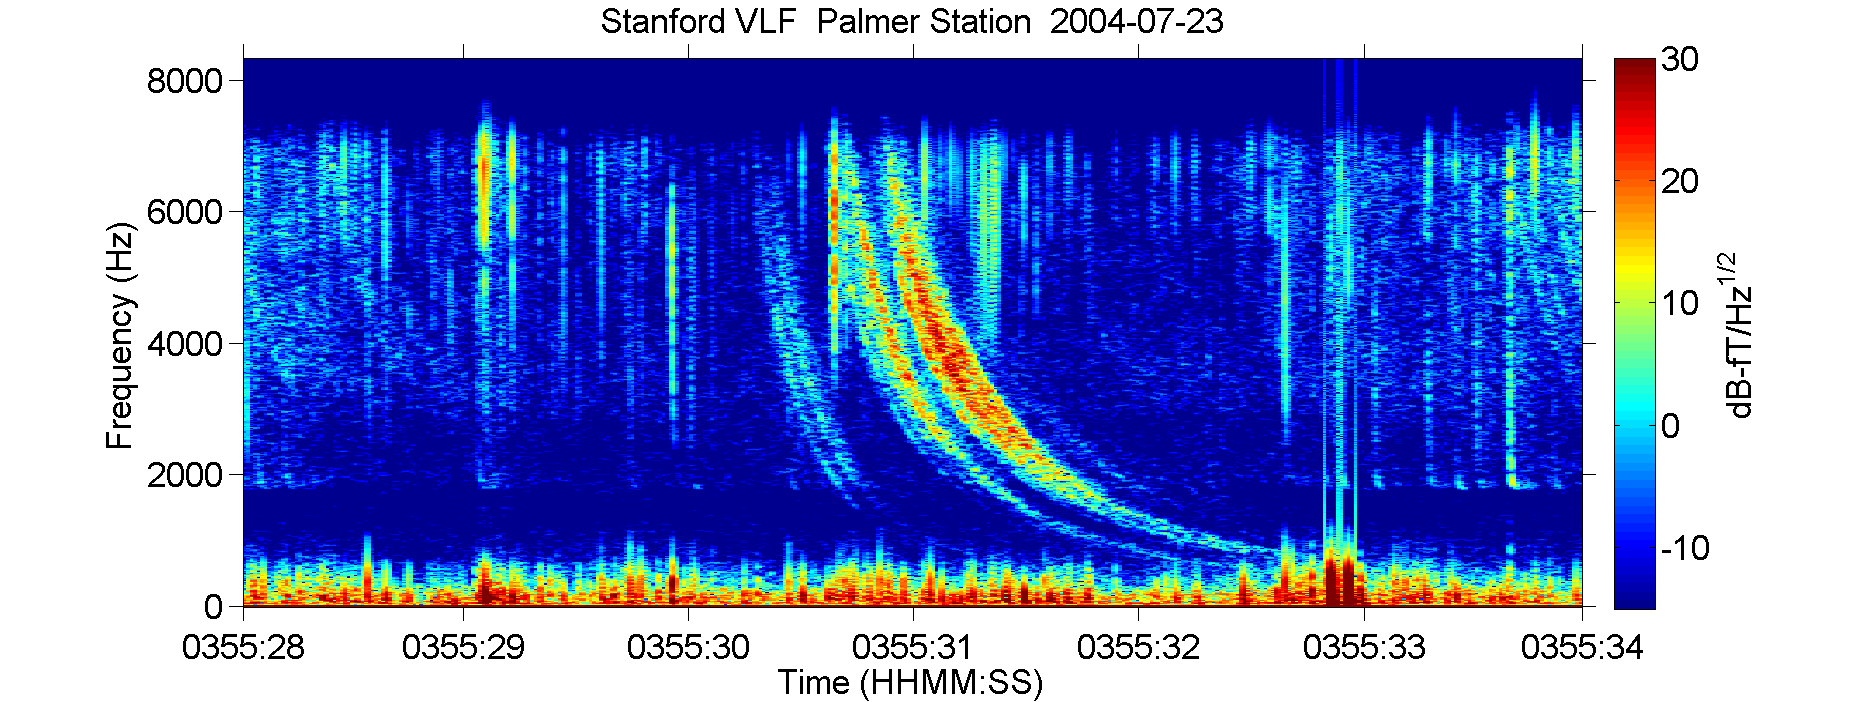
\includegraphics[width=1.0\textwidth,angle=0]{figures/chapter_2/whistler/Whistler_radio_palmer_2004-07-23_T035528.png}
\caption{Frequency/time relation for a typical whislter wave, observed by a Stanford University VLF radio receiver at Palmer Station, Antarctica.}
\end{figure}

A spectrogram showing how a typical whistler wave changes frequency in time is contained in Figure~\ref{whistler_spectrogram}, reproduced from data by the Stanford University VLF group. The radio receiver used to record these data were located at Palmer Station, Antarctica. The characteristic chirp decreasing in frequency is apparent. 

\subsection{Plasmaspheric Hiss}

Plasmaspheric hiss is a particular kind of whistler-mode wave which is responsible for the formation of the slot region in the radiation belts~\citep{lyons1972, lyons1973}. The frequency range is broadband ELF, occupying 100 Hz to a few KHz~\citep{millan2007}. The generation mechanism is not fully understood. Unlike whistler waves, plasmaspheric hiss shows no relation to lightning strikes at frequencies below 1 Khz~\citep{meredith04}. Theoretical modelling is consistent with generation by the electron cyclotron instability~\citep{millan2007, huang1983, church1983, meredith04}. The electron cyclotron instability, described by~\cite{thorne1979a}, was known in plasma physics before plasmaspheric hiss was discovered~\citep{kennel1966}, and is a way which whistler mode waves can change, amplify, and create his. At the time of writing, it is thought that there are several distinct mechanisms which combine to produce plasmaspheric hiss in different situations. Hiss below frequencies of 150 Hz is thought to be generated by amplification of whistler-mode noise due to substorm-injected electrons~\citep{meridith2018}. At higher frequencies, up to approximately 2 Khz, hiss likely comes from short bursts of chorus emissions (discussed in the next section), which exist farther out in space, propagate in, and become trapped in the plasmasphere~\citep{meridith2018}. Finally, at higher frequencies, hiss becomes more associated with land mass and geographic location, which suggests an association with terrestrial lightning. 

Debate about the origins of plasmaspheric hiss has spanned decades. Despite its clear importance with regards to the organization and stability of the radiation belts, it is not a process with a single, simple explanation. Modelling efforts, such as those by~\citep{meridith2018}, besides being useful descriptions in their own right, can help organize knowledge of the phenomenon into categories with different key drivers. Data from the Van Allen probe mission are still quite recent, and work is being undertaken (for example, that of~\cite{Li2015}) to create models based on these measurements. The best overall picture of plasmaspheric hiss is, currently, that a subset of chorus emissions (discussed in the next section) when they propagate from an equatorial source region to higher latitudes, become trapped within the plasmasphere, and merge together to form hiss~\citep{thorne2010,bortnick2008,bortnick2009}.

\subsection{Whistler Mode Chorus}

Chorus is a wave phenomenon consisting of discrete whistler-mode emissions, which are observed outside the plasmasphere, with a frequency range of 100 Hz to 5 Khz~\citep{millan2007}. The waves occur in two distinct bands, one below, and one above, half the electron gyrofrequency~\citep{Tsurutani1974,thorne2010}. It is believed that chorus is generated by the electron-cyclotron instability from injected plasma sheet electrons near the equator~\citep{kennel1966,millan2007}. When electrons are injected into the inner magnetosphere during active geomagnetic conditions, the instability results in wave amplification to non-high levels, in excess of 100 dB~\citep{li2008,li2009,thorne2010}. 

A primary reason for the importance of chorus waves is that they are a known cause of a phenomenon called microburst precipitation~\citep{millan2007}. Microburst precipitation is characterized by short, quasi-periodic bursts of electron precipitation that occur on timescales of 10 milliseconds. Microbursts were first discovered at relatively low energies (approximately 100 KeV), but they do occur at relativistic, MeV energies as well. The relation between microburst precipitation and chorus waves is suggested by the fact that they both predomenantly occur between 0300 and 1500 magnetic local time~\citep{lorentzen2001,millan2007}, and spacecraft measurements of both phenomena showed a strong correlation. An investigation by~\citet{thorne2005} used data from a 1998 geomagnetic storm event to estimate the miroburst precipitation rate due to whistler mode chorus waves and found general agreement between between observed, and model, loss rates at wave amplitudes consistent with observations~\citet{millan2007}.

Chrous waves are an important loss mechanism to the radiation belts. Pitch angle scattering caused by chorus waves occurs over a broad range of energies~\citet{thorne2010}, from tens of keV to MeV. There are limits to the applicability of the quasi-linear description of wave-particle interactions between electrons and chorus waves, which are relevant, because very large amplitude chorus waves have been observed, with electric field strengths of more than 240mV/m~\citep{cattell2008,thorne2010}. These cases, in particular, highlight the need for experimental measurements as constraints for implemented models. 

\subsection{Electron Ion Cyclotron (EMIC) Waves}

EMIC waves are a distinct type of electromagnetic wave, which occur at frequencies in bands separated by multiples of the ion gyrofrequency~\citep{thorne2010}. Differnt ion species give rise to different frequencies for EMIC waves. These waves are thought to originate near the equator~\citep{fraser1996,lotouaniu2005,millan2007}, where they are created by a temperature anisotropy in the ring current with respect to the local magnetic field~\citep{jordanova2001}. EMIC waves are known to be a major source of loss for electrons in the radiation belts. At energies of greater than approximately several 100 keV, they are effective at scattering electrons into the loss cone~\citet{thorne1981,millan2007}.The resonance condition requires that the wave, which is left-hand circularly polarized, be seen in the electron frame as right-hand polarized. This happens when the electron overtakes the wave, and so requires the electrons to have a  minimum energy~\citet{millan2007}. This minimum energy required can be calculated from the dispersion relation of the EMIC wave.

Balloons and satellites are two complementary ways which electron precipitation has been measured. Satellite observations suggest that, most of the time, precipitation caused by EMIC waves occurs at higher energies~\citep{millan2007}. The survey conducted by~\citep{merideth2003} using measurements of EMIC waves by the CERES satellite found that the resonant energy required for electron scattering was less than 2 MeV in only approximately 11 percent of cases. The first balloon with a detector capable of measuring these higher energies was flown from 1996 in Kiruna, Sweden~\citep{millan2007}. This balloon measured electron precipitation with a peak characteristic energy of 1.7 MeV~\citep{foat1998}. The observed precipitation was later shown by~\citep{lorentzen2000} to be associated with nearby spacecraft observations of EMIC waves~\citet{millan2007}.


\subsection{Anatomy of Wave Particle Interactions and Geospace}

Geospace has a structure, explained and quantified through measurements, in which different wave and scattering phenomenon are active. A loose analogy can be drawn between this overall system and the anatomy of a living thing, such as a cell. Figure~\ref{anatomy}, reproduced from~\citet{thorne2010}, shows the relevant structure at this level of detail. Particle drift motions are overlaid with sketches of regions and their primary associated waves. The Earth is shown as a brown sphere in the middle of the figure. The projection is looking downwards at the equatorial plane. 

The geometry and regions are essentially controlled by a combination of the Earth's magnetic field and the magnetic field carried by the solar wind. The magnetopause, which is the boundary between solar wind plasma and plasma associated with the near-Earth environment, defines the extent of the map. In the plasmasphere, where plasma densities are relatively dense, plasmaspheric hiss is found. The source region is equatorial, and the waves propagate to higher latitudes~\citep{thorne2010}. Within this region, the plasma is relatively cold and dense. An order-of-magnitude drop in plasma density defines the outward extend of the region. 

Azimuthal drift of the bounce motion, occurs in different directions for ions and electrons, and forms the ring current. Whistler-mode chorus waves exist in this lower density region, along with classic whistlers, which more or less follow the geometry of the Earth's magnetic field lines and can bounce between magnetically conjugate points. EMIC waves, on the other hand, have a favored region which lies between where the plasmasphere and the ring current overlap~\citep{thorne2010}.

As electrons undergo bounce motion, all of these wave phenomena together can scatter them into the loss cone, causing them to be lost to the atmosphere on a subsequent bounce. All of the different components of this combined system share information via the exchange of energy, and momentum through wave particle interactions. Because of this, it is important to develop techniques which can extract information from the accessible parts of the system. This is the goal which will be discussed in subsequent chapters.  

\clearpage
\begin{figure}[h!]
\label{anatomy}
\centering
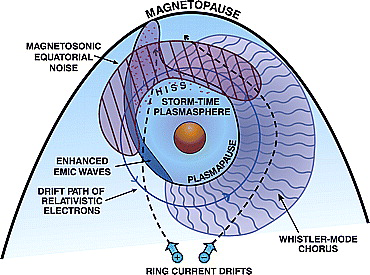
\includegraphics[width=1.0\textwidth,angle=0]{figures/chapter_2/anatomy/anatomy.png}
\caption{Overall structure and layout of wave activity and particle drifts in near-Earth space, reproduced with permission from~\citet{thorne2010}.}
\end{figure}
\newpage
\section{Particle Precipitation as Information Transport}

The wave phenmomena discussed in this chapter are distinct, but are also related. There is no single, simple, and unifying description for them all. The state of knowledge of the wave-particle interactions which occur in near-earth space has advanced over the course of decades, but work still remains to be done. It can be described at this stage as a mix of phenomenological descriptions, experimental data, and models which attempt to reproduce specific components, subject to experimental constraints. Despite the fact that this field of study is complicated, there is one relatively simple fact that unifies the different wave-particle interactions: that they are energy selective. The nature of resonance conditions requires this, and so, when measurements of the particles themselves are either avaialble, or their properties are able to be inferred, it provides a window into the proccesses in broader geospace.

The focus of this thesis is on one particular technique which can be used to obntain knowledge about one fraction of the particles in the system. While as far as the magnetospheric physics is concerned, the story of the precipitating electrons ends once they are scattered into the loss cone and undergo their final bounce motion in the magnetic surroundings of the Earth, they carry information down into the atmosphere, where they can be more easily observed. Once entry into the Earth atmosphere occurs, the secondary radiation released by the electrons, mostly in the form of X-rays, penetrates deeply enough to be directly measured by balloon-borne detectors. 
 The retrieval of the information that the electrons carry is the problem which will be examined in the following chapters. It will be shown that the problem of obtaining the maximum information with the fewest restrictive assumptions leads to some interesting problems, but that ultimately, the indirect measurement of electron precipitation can provide a window in to the properties of the scattered population in space, a task which is complementary to the view provided by orbiting satellites. 
